\chapter{Contribution}
Spatial filtering is a form of finite impulse response (FIR) filtering. The filter is a mask of weights arranged
in a rectangular pattern. It mean that sliding the mask along the image and performing a multiply and
accumulate operation on the pixels covered by the mask.

\section*{Original Image }
First, we are going to read and show original image as below :
\begin{lstlisting}
I = imread('lena.tif');
F = imshow(I);
\end{lstlisting}

\textbf{Result:}
\begin{center}
	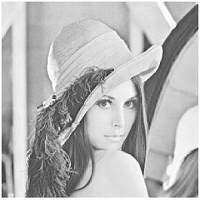
\includegraphics{lena1.png}

 Original Image
\end{center}

\section{Median Filter}
Median Filter is family of order filters. It has process : Replace the value of a pixel with the median value of the neighborhood.

$I_{median} = median(I[i,j])$  with $(i,j)\in neighborhood$

From theory above, we are going to build function for median filter :

\begin{lstlisting}
function F = median(I,w)
s=size(I);
for i=floor(w/2)+1:s(1)-floor(w/2)
	for j=floor(w/2)+1:s(2)-floor(w/2)
		for k=1:w
			for l=1:w
				vect(w*(k-1)+l)=I(i-floor(k/2)+2,j-floor(l/2)+2);
			end
		end
		B=sort(vect);
		I(i,j)=B(floor(size(B,2)/2)+1);
	end
end
figure;

imshow(I);

\end{lstlisting}


\textbf{Result:}

\begin{center}
	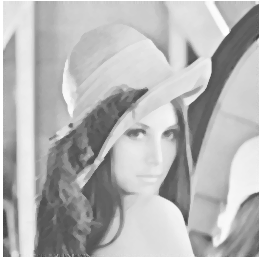
\includegraphics{median1.png}
	
	median x 7
\end{center}

\section{Average Filter}

\

Feature: 

\

A spatial filter that applies to a neighborhood (local method).

\

A linear filter, speaking as a convolution.

\

A pixel is replaced by the average of itself and its neighbours.

\

The neighborhood size determines the amount of smoothing.

\

Equivalent to a filtering operation lowpass.

\

Average Filter have: 
\begin{center}
	Filter 3$\times$3

$\dfrac{1}{9}\begin{tabular}{|c|c|c|}
\hline 
1 & 1 & 1 \\ 
\hline 
1 & 1 & 1 \\ 
\hline 
1 & 1 & 1 \\ 
\hline 
\end{tabular}$ 	
\end{center}

\

\begin{center}
		Filter 5$\times$5
	
	$\dfrac{1}{25}\begin{tabular}{|c|c|c|c|c|}
		\hline 
		1 & 1 & 1 & 1 & 1 \\ 
		\hline 
		1 & 1 & 1 & 1 & 1 \\ 
		\hline 
		1 & 1 & 1 & 1 & 1 \\ 
		\hline 
		1 & 1 & 1 & 1 & 1 \\ 
		\hline 
		1 & 1 & 1 & 1 & 1 \\ 
		\hline 
	\end{tabular} $
\end{center}

\

\begin{center}
	Filter 7$\times$7

$\dfrac{1}{49}\begin{tabular}{|c|c|c|c|c|c|c|}
	\hline 
	1 & 1 & 1 & 1 & 1 & 1 & 1 \\ 
	\hline 
	1 & 1 & 1 & 1 & 1 & 1 & 1 \\ 
	\hline 
	1 & 1 & 1 & 1 & 1 & 1 & 1 \\ 
	\hline 
	1 & 1 & 1 & 1 & 1 & 1 & 1 \\ 
	\hline 
	1 & 1 & 1 & 1 & 1 & 1 & 1 \\ 
	\hline 
	1 & 1 & 1 & 1 & 1 & 1 & 1 \\ 
	\hline 
	1 & 1 & 1 & 1 & 1 & 1 & 1 \\ 
	\hline 
\end{tabular} $
\end{center}
\vspace{1cm}


\begin{lstlisting}
function F=average(I)
s=size(I);
F_size=7;
F=double(zeros(s(1),s(2)));
	for i=floor(F_size/2)+1:s(1)- floor(F_size/2)
		for j=floor(F_size/2)+1:s(2)- floor(F_size/2)
			for k=1:F_size
				for l=1:F_size
					F(i,j)=F(i,j)+double(I(i+k-(floor(F_size/2)+1),j+l-(floor(F_size/2)+1)));
				end;
			end;
			F(i,j)=round(F(i,j)/(F_size*F_size));
			end;
		end;
F=uint8(F);
figure;
imshow(F);
\end{lstlisting}



\textbf{Result:}

\begin{center}
	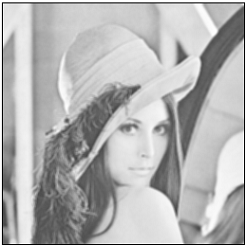
\includegraphics{a3x3.png}
	
	Filter $3\times3$
	
	 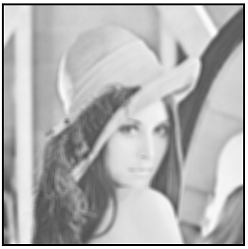
\includegraphics{a5x5.png}
	
	Filter $5\times5$
	
		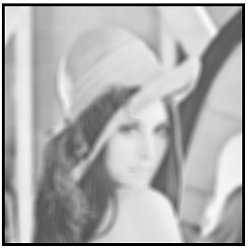
\includegraphics{a7x7.png}
	
Filter $7\times7$
\end{center}

\section{Gaussian Filter}

The Gaussian kernel in dimension 2:


$G(x,y) = \dfrac{1}{2\pi\sigma^2}\exp\left[-\dfrac{(x-\mu_x)^2+(y-\mu_y)^2}{2\sigma^2}\right ]$

\

Define the Gaussian mask:
%$$\mu = 0$$
%$$\sigma = 0.8$$
\begin{center}
	Filter 3$\times$3

$\dfrac{1}{16}\begin{tabular}{|c|c|c|}
	\hline 
	1 & 2 & 1 \\ 
	\hline 
	2 & 4 & 2 \\ 
	\hline 
	1 & 2 & 1 \\ 
	\hline 
\end{tabular} $
\end{center}

\begin{center}
	Filter 5$\times$5

$\dfrac{1}{273}\begin{tabular}{|c|c|c|c|c|}
	\hline 
	1 & 4 & 7 & 4 & 1 \\ 
	\hline 
	4 & 16 & 26 & 16 & 4 \\ 
	\hline 
	7 & 26 & 41 & 26 & 7 \\ 
	\hline 
	4 & 16 & 26 & 16 & 4 \\ 
	\hline 
	1 & 4 & 7 & 4 & 1 \\ 
	\hline 
\end{tabular}$ 
\end{center}

\begin{center}
	Filter 7$\times$7

$\dfrac{1}{1003}$\begin{tabular}{|c|c|c|c|c|c|c|}
	\hline 
	0 & 0 & 1 & 2 & 1 & 0 & 0 \\ 
	\hline 
	0 & 3 & 13 & 22 & 13 & 3 & 0 \\ 
	\hline 
	1 & 13 & 59 & 97 & 59 & 13 & 1 \\ 
	\hline 
	2 & 22 & 97 & 159 & 97 & 22 & 2 \\ 
	\hline 
	1 & 13 & 59 & 97 & 59 & 13 & 1 \\ 
	\hline 
	0 & 3 & 13 & 22 & 13 & 3 & 0 \\ 
	\hline 
	0 & 0 & 1 & 2 & 1 & 0 & 0 \\ 
	\hline 
\end{tabular} 
\end{center}



From theory above, we are going to build function for gaussian filter :
%\begin{lstlisting}
%function F = gaussian(I) 
%s=size(I);
%F_G=[1,2,1;2,4,2;1,2,1];
%F_size=3;
%F=double(zeros(s(1),s(2)));
	%for i=2:s(1)-1
		%for j=2:s(2)-1
			%for k=1:3
				%for l=1:3
					%F(i,j)=F(i,j)+double(I(i+k-2,j+l-2)*F_G(k,l));
					%end;
				%end;
					%F(i,j)=round(F(i,j)/(16));
				%end;
			%end;
%F=uint8(F);
%figure;
%imshow(F)
%\end{lstlisting}
\begin{lstlisting}
% Read an image
I = imread('lena.tif');
% Create the gaussian filter with hsize = [x y] and sigma = 2
G = fspecial('gaussian',[x y],2);
% Filter it
F = imfilter(I,G,'same');
% Display
imshow(F)	
\end{lstlisting}
\textbf{Result:}
\begin{center}
	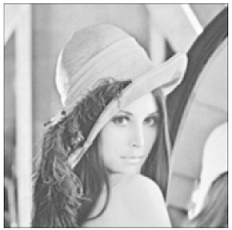
\includegraphics{b3x3.png}
	
	Filter $3\times3$
	
	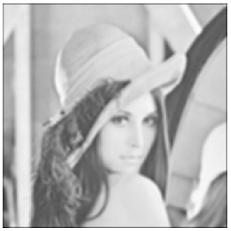
\includegraphics{b5x5.png}
	
	Filter $5\times5$
	
	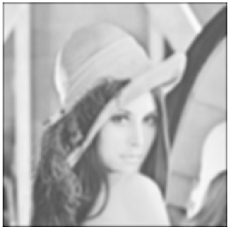
\includegraphics{b7x7.png}
	
	Filter $7\times7$
\end{center}
\newpage
\section{Wiener Filter}

%Weiner filter are characterized by following:
%\begin{itemize}
%	\item Assumption: Signal and additive noise are stationary linear with known spectral characteristics or known autocorrelation and cross-correlation.
%	\item Requirement: the filter must be physically realizable.
%	\item Performance criterion: minimum mean –square error. 
%\end{itemize} 

\begin{lstlisting}
%Add noise
subplot(2,2,1);
I = imread('lena.tif');
J = imnoise(I,'gaussian',0,0);
imshow(J(100:256,1:256));
title('Added Gaussian Noise');

%Remove noise
subplot(2,2,2);
K = wiener2(J,[5 5]);
D = imshow(K(100:256,1:256));
title('Noise Removed by Wiener Filter');
\end{lstlisting} 

\textbf{Result:}
\vspace{1cm}
\begin{center}
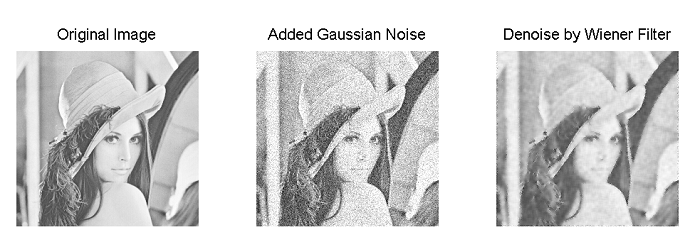
\includegraphics{Wiener.png}
\end{center}


%In this part, you must explain your proposition to solve/address the problematic explained in the introduction chapter.\\

%You must be as clear  as possible, and you must use classical formalizations (Mathematical, software model, hardware model, Uml, etc) to explain 
%your method/algorithm/system.




